\documentclass[12pt,a4paper]{article}
\usepackage{enumitem}
% Define margins
\setlength{\topmargin}{-1.0cm}
\setlength{\oddsidemargin}{0.1cm}
\setlength{\textwidth}{16.5cm}
\setlength{\textheight}{23.0cm}

% Use Times New Roman font
\usepackage{times}
\usepackage{xurl}
\usepackage{url}
\usepackage[hidelinks]{hyperref} 
\urlstyle{rm}

\renewcommand{\rmdefault}{ptm}

\usepackage{graphicx} % LaTeX package to import graphics
\graphicspath{{images/}} % Configuring the graphicx package

% Define header and footer
\usepackage{fancyhdr}
\pagestyle{fancy}
\fancyhf{}
\rhead{\textbf{\textit{Week 6 Submission}}}
\cfoot{\textbf{\textit{\thepage}}}
\renewcommand{\headrulewidth}{0.7pt}
\setlength{\headheight}{14pt}

% Adjust section and subsection title formats
\usepackage{titlesec}
\titleformat{\section}
  {\normalfont\fontsize{14}{15}\bfseries}{\thesection}{1em}{}
\titleformat{\subsection}
  {\normalfont\fontsize{12}{15}\bfseries}{\thesubsection}{1em}{}

% Define a style with no footer for the table of contents
\fancypagestyle{nofooter}{%
  \fancyfoot{}%
}

% To manage references
\usepackage{natbib}
\usepackage[labelfont=bf]{caption}

\begin{document}

% TITLE PAGE

\begin{titlepage}

\newcommand{\HRule}{\rule{\linewidth}{0.5mm}}
\center

\vspace*{1\baselineskip}

\includegraphics[width=0.15\textwidth]{images/UTS.png}\\
\textsc{\LARGE University of Technology Sydney}\\[2.0cm]
\textsc{\Large (32557) Enabling Enterprise Information Systems}\\[0.4cm]

\HRule\\[0.6cm]
{\huge\bfseries Design Thinking \& IS-Enabled Solutions (Part 1) }\\[0.4cm]
\HRule\\[10cm]

\emph{by Team Super} \\
{ Seoyoon Kim (25388442) [Group leader] \\}
{ Jin Lee (25388733)  \\}
{ Ariel Manueke (25207919) \\}
{ Nonthawat Praisompong (25233750) \\}

\vfill
{\large\today}

\vfill

\end{titlepage}

% TABLE OF CONTENTS

\tableofcontents
\thispagestyle{nofooter}
\cleardoublepage

\pagebreak

% DOCUMENT CONTENT STARTS HERE
% You can start writing your document content here.


% Student %%%%%%%%%%%%%%%%%%%%%%%%%%%%%%%%%%%%%%%%%%%%%%%%%%%%%%%%%%%%%%%%%%%%%%%%%%%%%%%%%%%%%%%%%

\setcounter{page}{1}

\section{Question 1}
\subsection{Qantas Efforts to Help Solve Social Problems in Accordance with the UN Sustainable Development Goals.}

Our team chose Qantas, the national airline of Australia, which is also the second-oldest passenger airline in the world, established in 1920 \citep{Ref1.1}. Qantas has been a major player in the Australian aviation industry connecting the Australian continent to the major parts of the world, including their ambitious project sunrise plan to operate the longest passenger flight in the world from Sydney to London that will take over 19 hours directly \citep{Ref1.2}. Being the pride of Australian airlines, Qantas has gained a popular image using its Australian flagship animal which is the kangaroo as its prime logo, getting them the nickname of flying kangaroo \citep{Ref1.3}.\\ 

\noindent Since its establishment over a century ago, Qantas as a flight service provider, also has tried to embed some of the social problems related to the UN’s Sustainable Development Goals (SDG). The first goal of SDG is the 3rd goal which is the good health and wellbeing, where Qantas launched their Qantas Wellbeing App (QWA) that can be downloaded from a customer’s smartphone to be able to earn the airline’s Qantas frequent flyer points while doing some healthy lifestyle such as workouts, shopping, and other daily activities as shown in Figure 1 \citep{Ref1.4}. A research about QWA shows that the app successfully turns the everyday activity of its user’s life into collecting data and manipulation in exchange for earning points \citep{Ref1.5}. \\

\begin{figure}[htbp]
    \centering
    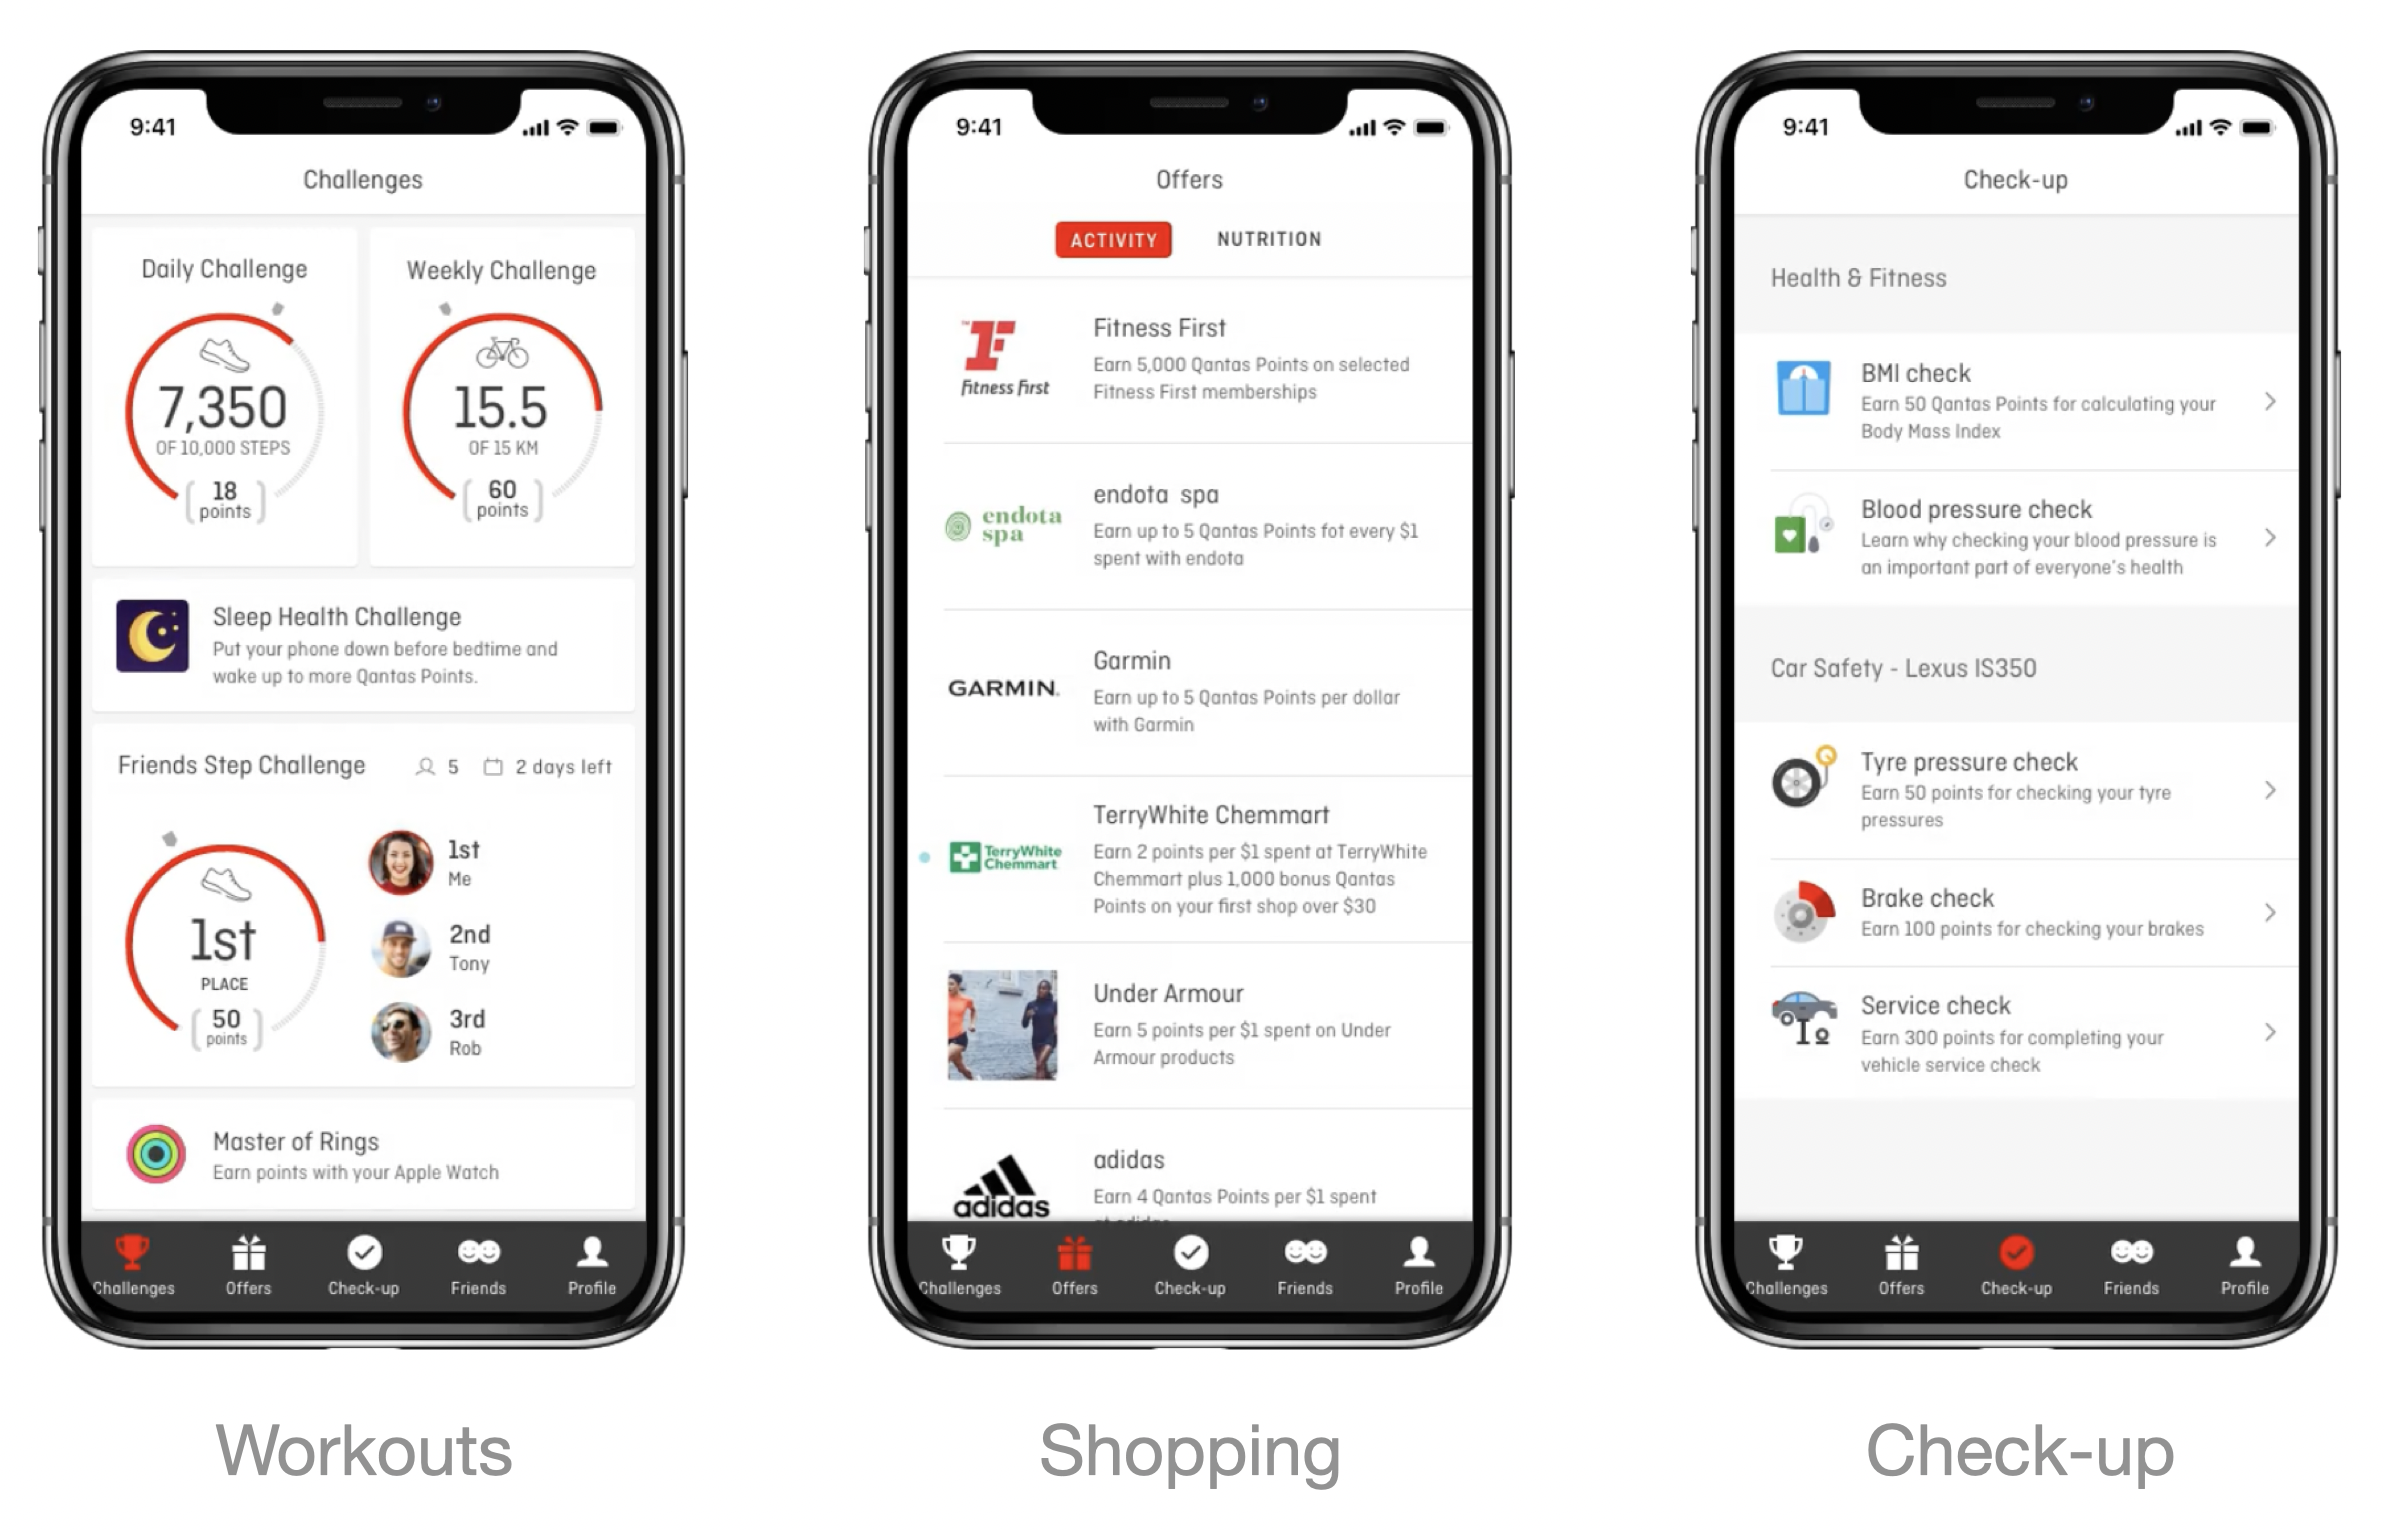
\includegraphics[width=0.8\textwidth]{images/Qantas Wellbeing App.png}
    \caption{Qantas wellbeing app \citep{Ref1.4}}
    \label{fig:example}
\end{figure}

\noindent Another SDG goal that Qantas has tried to help, as a flight service provider, is the 7th goal which is the affordable \& clean energy. Qantas has been working to reach its goal, as a major player in the aviation industry, of reducing carbon emissions significantly by implementing several efforts such as making passengers contribute to the sustainability of ticket costs, investing in sustainable fuel, increasing its fuel efficiency with the latest advanced aircraft, and reducing junkyard contribution by removing plastic cutlery. Although Qantas has been making significant progress with multiple successful environmental practices, this goal is a long-term and ambitious project that still needs prolonged effort to reach its goal for net-zero emission goal \citep{Ref1.6}. \\ 
\pagebreak%%%%%%%%%%%%%%%%%%%%%%%%%%%%%%%%%%%%%%%%%%%%%%%%%%%%%%%%%%%%%%%%%%%%%%%%%%%%%%

\setcounter{page}{3}

\section{Question 2}
\subsection{Report on Addressing Operational Challenges at Qantas Airways }
\label{sec:Question 2}
\textbf{Objective:}\\
\noindent To brainstorm and identify potential solutions for improving flight delays, addressing pilot shortages, optimizing delay performance, and enhancing the cancellation point refund policy at Qantas Airways to improve overall customer satisfaction.\\

\noindent\textbf{Identified Issue/Problem:}\\
\noindent Qantas Airways is grappling with operational challenges that include significant flight delays, a shortage of pilots leading to cancellations, inadequate delay performance measures, and customer dissatisfaction stemming from the existing cancellation point refund policy \citep{Ref2.1}. These issues not only affect passengers but also have wider implications for the company’s staff, partners, and the airline industry at large \citep{Ref2.2}. \\

\noindent\textbf{Stakeholders: }
\begin{itemize}
    \item \textbf{Passengers:} The primary affected group, experiencing inconvenience and disruptions to their travel plans.
    \item \textbf{Pilots and Airline Staff:} Their schedules, job satisfaction, and workload are directly impacted by operational inefficiencies.
    \item \textbf{Qantas Management and Shareholders:} Interested in maintaining profitability, brand reputation, and customer loyalty.
    \item \textbf{Airport Operators and Vendors:} Depend on efficient airline operations for their business activities and customer service.
    \item \textbf{Travel Agencies and Partner Airlines:} Rely on Qantas for reliable scheduling and services for their customers.
    \item \textbf{Regulatory Authorities:} Ensure airlines comply with consumer protection laws and safety regulations.
\end{itemize}

\noindent\textbf{Brainstormed Ideas for Solutions: }
\begin{itemize}
  \item \textbf{Expanding Pilot Recruitment and Training:} 
    \begin{itemize}
      \item Invest in targeted recruitment campaigns and partnerships with aviation schools to address the pilot shortage. 
      \item Enhance training programs to fast-track the readiness of new pilots and upskill existing staff. 
    \end{itemize}
  \item \textbf{Optimizing Flight Schedules:} 
    \begin{itemize}
      \item Implement advanced predictive analytics to optimize flight schedules and minimize delays.
      \item Develop a more robust system for managing and adjusting flight schedules in real-time to respond to unforeseen challenges. 
    \end{itemize}
    \item \textbf{Improving Communication Strategies:} 
    \begin{itemize}
      \item Establish a comprehensive communication strategy to keep passengers informed about delays, cancellations, and alternatives in real-time. 
      \item Use mobile app notifications, social media, and the airline's website to provide updates and manage passenger expectations effectively. 
    \end{itemize}
    \item \textbf{Revamping the Cancellation Point Refund Policy:} 
    \begin{itemize}
      \item Introduce a more transparent and customer-friendly refund policy that provides clearer options for points refund or rebooking.
      \item Offer additional compensation or benefits for significant inconveniences to enhance customer loyalty. 
    \end{itemize}
    \item \textbf{Investing in Technology and Infrastructure:}  
    \begin{itemize}
      \item Upgrade technological infrastructure to support more efficient operations, including scheduling, staffing, and customer service.
      \item Leverage AI and machine learning for predictive maintenance to reduce aircraft downtime and avoid delays. 
    \end{itemize}
\end{itemize}
 

\noindent\textbf{Conclusion:}\\
\noindent Addressing the operational challenges at Qantas Airways requires a multifaceted approach that involves improving internal processes, investing in technology, and focusing on customer service excellence. By implementing the brainstormed ideas, Qantas can enhance its operational efficiency, reduce flight delays and cancellations, and improve customer satisfaction and loyalty. Engaging with all stakeholders and considering their perspectives and needs is crucial for developing and implementing effective solutions to these complex challenges. \\


\pagebreak
%%%%%%%%%%%%%%%%%%%%%%%%%%%%%%%%%%%%%%%%%%%%%%%%%%%%%%%%%%%%%%%%%%%%%%%%%%%%%%

\setcounter{page}{5}

\section{Question 3}
\subsection{Empathy Map of Flight Travel of Customers}
\label{sec:Question 3}
\begin{figure}[htbp]
    \centering
    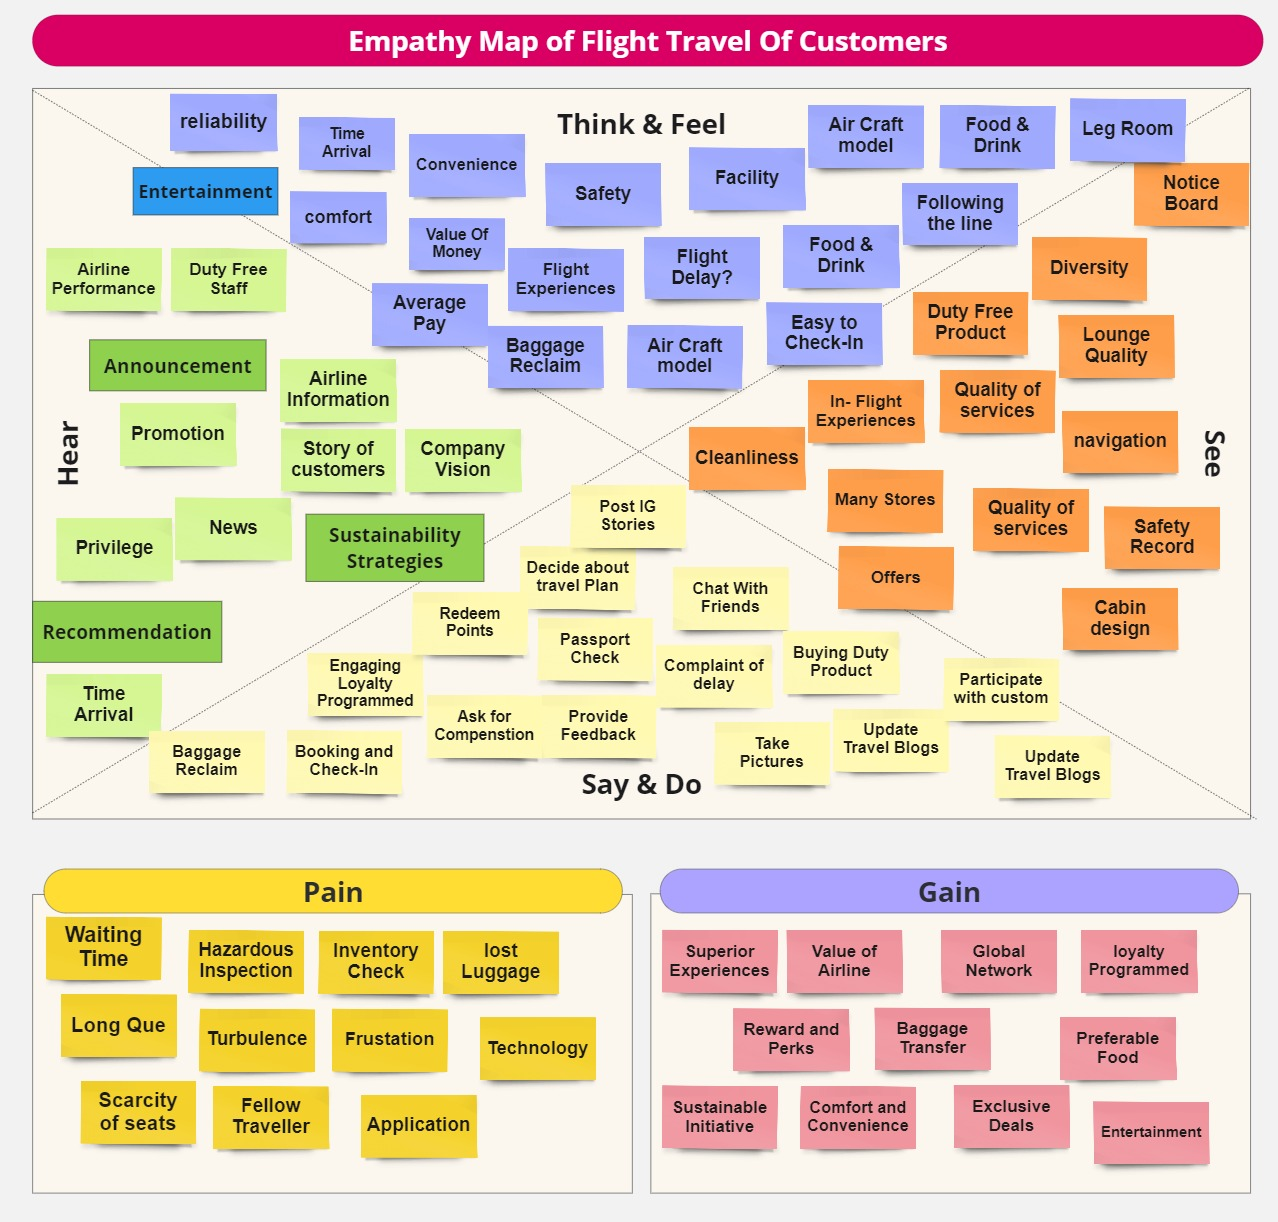
\includegraphics[width=1.0\textwidth]{Customer Touchpoint Map.jpg}
    \caption{Empathy Map Result}
    \label{fig:example}
\end{figure}



\pagebreak
% BIBLIOGRAPHY %%%%%%%%%%%%%%%%%%%%%%%%%%%%%%%%
 

% Use Leeds Harvard referencing template
\bibliographystyle{lsharvard}
% Add here the bib file with your references
\bibliography{references}
	
\def\UrlBreaks{\do\/\do-}

\clearpage
\end{document}
